\section{eo\-Stdout\-Monitor Class Reference}
\label{classeo_stdout_monitor}\index{eoStdoutMonitor@{eoStdoutMonitor}}
Prints statistics to stdout.  


{\tt \#include $<$eo\-Stdout\-Monitor.h$>$}

Inheritance diagram for eo\-Stdout\-Monitor::\begin{figure}[H]
\begin{center}
\leavevmode
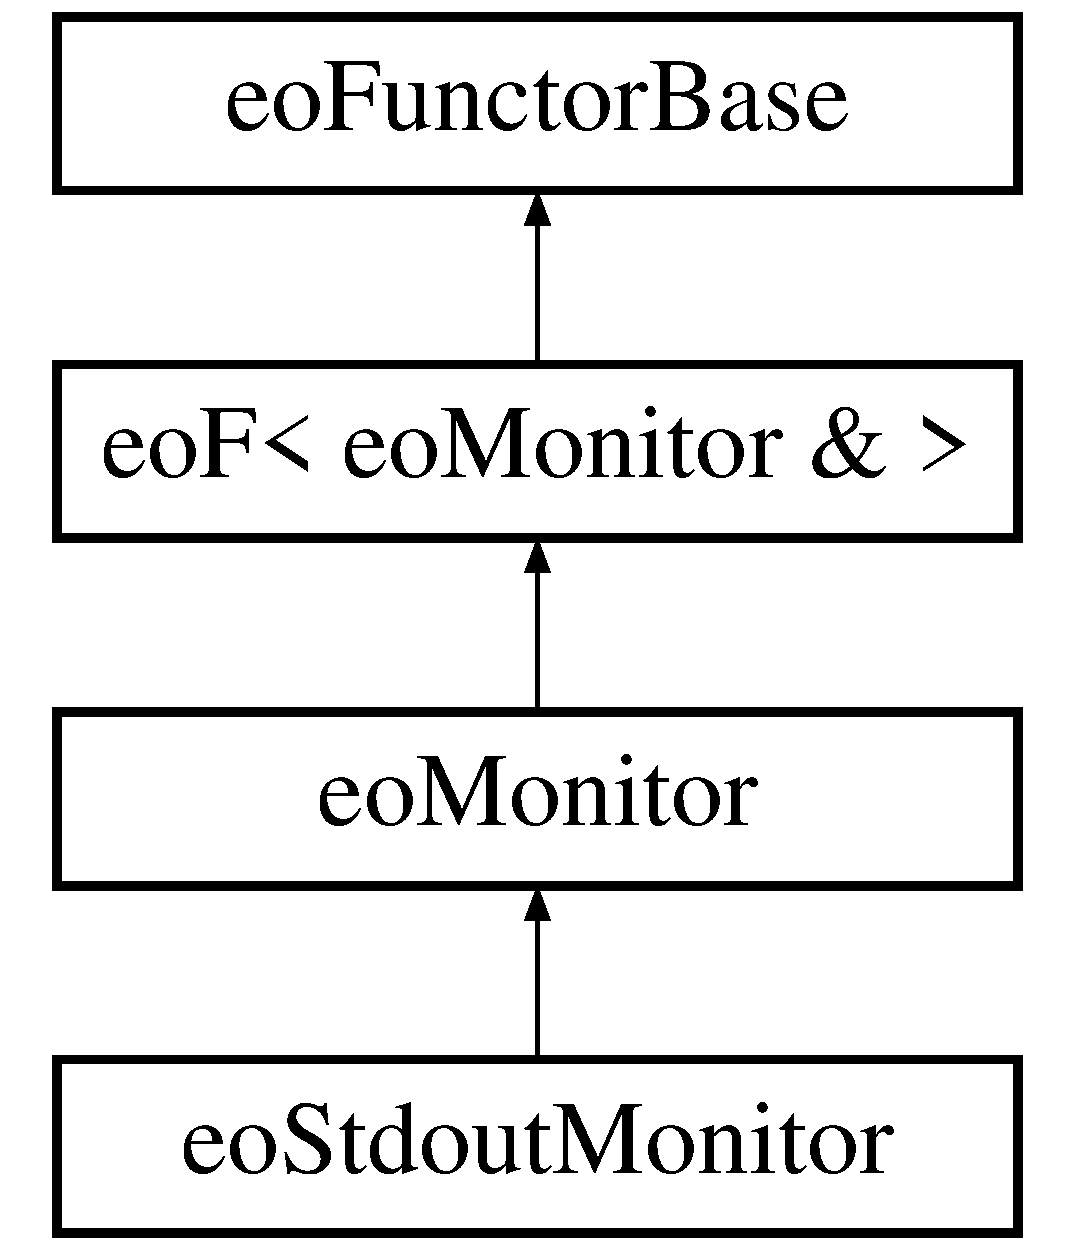
\includegraphics[height=4cm]{classeo_stdout_monitor}
\end{center}
\end{figure}
\subsection*{Public Member Functions}
\begin{CompactItemize}
\item 
{\bf eo\-Stdout\-Monitor} (bool \_\-verbose=true, std::string \_\-delim=\char`\"{}$\backslash$t\char`\"{})\label{classeo_stdout_monitor_a0}

\item 
{\bf eo\-Monitor} \& {\bf operator()} (void)\label{classeo_stdout_monitor_a1}

\begin{CompactList}\small\item\em The pure virtual function that needs to be implemented by the subclass. \item\end{CompactList}\item 
virtual std::string {\bf class\-Name} (void) const \label{classeo_stdout_monitor_a2}

\end{CompactItemize}
\subsection*{Private Attributes}
\begin{CompactItemize}
\item 
bool {\bf verbose}\label{classeo_stdout_monitor_r0}

\item 
std::string {\bf delim}\label{classeo_stdout_monitor_r1}

\item 
bool {\bf firsttime}\label{classeo_stdout_monitor_r2}

\end{CompactItemize}


\subsection{Detailed Description}
Prints statistics to stdout. 



Definition at line 38 of file eo\-Stdout\-Monitor.h.

The documentation for this class was generated from the following files:\begin{CompactItemize}
\item 
eo\-Stdout\-Monitor.h\item 
eo\-Stdout\-Monitor.cpp\end{CompactItemize}
